%============================================================
\section{Nombre: Lluvia de huesos.}\label{hab.LluHuesos}
\subsection{Descripción}
Caen huesos del cielo en posiciones aleatorias. Los huesos se destruyen al colisionar con el suelo, con una plataforma o con el jugador. Cuando una de los huesos colisiona con el jugador disminuye la cantidad de vida del jugador, es decir cada hueso genera daño de manera individual. Los huesos no pueden destruir las plataformas o el suelo al colisionar contra estas.
\subsection{Portador}
Mictlantechtli (ver apartado \ref{per:mictlantechtli}).	
\subsection{Esquema}
			Ver figura \ref{fig:penitencia}.
			\begin{figure}
				\centering
				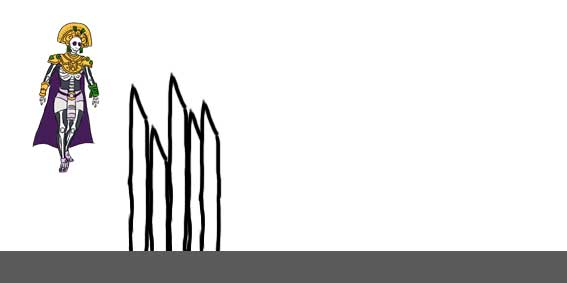
\includegraphics[height=0.2 \textheight]{Imagenes/penitencia}
				\caption{Penitencia.}
				\label{fig:penitencia}
			\end{figure}